% !TEX root = ../thesis.tex
%
\chapter{Related Work}
\label{sec:review}

% \cleanchapterquote{"Mens cujusque is est Quisque" ¨C "Mind Makes the Man"}{Samuel Pepys}{}

% \blindtext
% 2. Related work
% (1) Blockchain, in particular Ethereum; (2) Transaction analysis; (3) Visualization for Blockchain; (4) Difference between your work and existing studies.

\section{Ethereum Transactions}
\label{sec:review:transactions}

% \blindtext
In the simplest terms, blockchain represents an unchangeable digital ledger system. A distinctive feature of blockchain technology is its distributed implementation, further discussions on blockchain can be found in many publications \cite{9}. Bitcoin blockchain is one of the best known blockchains for speculation in Bitcoin cryptocurrency and payments with Bitcoin wallets. Ethereum blockchain is another popular blockchain for executing complex transactions on top of transferring value in its cryptocurrency Ether. It allows to create smart contracts and enables users to create crypto-assets. For example, Ethereum tokens are sold in the event of Initial Coin Offering (ICO) \cite{10}. Such token ICOs have attracted many startups and organizations to raise funds by selling digital coins that allow recipients to use the promised service as much as possible. In the years of 2018 and 2019, Ethereum ICO raised billions of dollars. While fluctuations in Ether prices are not Ethereum transactions, ICO is a process involving many Ehtereum transactions.

\begin{figure}[htb]
	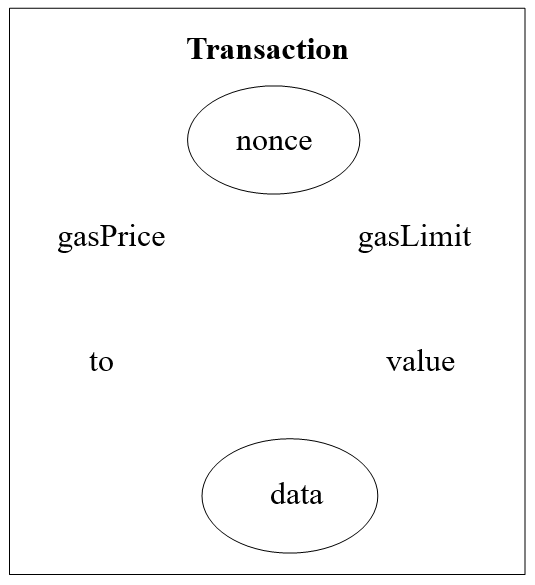
\includegraphics[width=0.7\textwidth]{gfx/transactions.png}
	\caption{Example of an External Transaction}
	\label{fig:transactions}
\end{figure}

Ethereum is a state machine based on transactions. In other words, a transaction occurred between two different accounts converts Ethereum globally from one state to another \cite{13}. A transaction is executed in a block, its two accounts are the source and target. These accounts can be Externally Owned Accounts (EOAs) or smart contracts, EOAs are serialized and then submitted to the blockchain. There are two types of transactions including external transactions and internal transactions. In an external transaction, the sender (source) account is an EOA, the recipient (target) account is an EOA if the transaction is money transfer or it is a contract account if the transaction is contract creation or contract invocation \cite{14}. The data fields of an external transaction include account addresses, timestamp, value and others \cite{16}. The Fig. \ref{fig:transactions} shows typical elements of an external transactions. For an internal transaction, the source account is smart contract instead of EOA, its corresponding activities are transferring money to EOA, creating smart contract and invoking smart contract which are the same for an external transaction. Every account has a nonce keeping track of the transactions they perform, it can be used to prevent replay attacks. A transaction is a list of operations to be executed, gas for an operation is relatively fixed and required to perform this operation. The gasPrice field represents the price per unit of gas you are willing to pay while the gasLimit field determines how many units of gas you are willing to pay for.

\section{Evolution Analysis}
\label{sec:review:evolution}

% \blindtext
Regarding transaction analysis, Chen et al. analyze all the Ethereum transactions from 30 Jul 2015 to 10 Jun 2017 by constructing Money Flow Graph (MFG) for money transfer, Contract Creation Graph (CCG) for smart contract creation and Contract Invocation Graph (CIG) for smart contract invocation \cite{3}. They also provide graph analytics as measures of degree, clustering, correlation, importance, assortativity and connected components. Yue et al. develop a web application called BitExTract for interactive visualization of Bitcoin exchanges, it provides views including exchanges list panel for selecting exchanges, massive sequence view for related news, connection view for inter-exchange relationships grouped by geographical region and comparison view for transaction amounts over time \cite{19}. It is worth noting that it enables users to select exchanges and time interval, which gives users flexibility to extract information about evolution of Bitcoin exchanges.

Regarding graph visualization, Lanum suggests Gephi which is a Graphical User Interface (GUI) written in Java for building graph visualization, it provides many options for configuring its built-in UI \cite{4}. Meanwhile, there is a considerable learning cost of these Gephi-specific configurations, and the manual process of data handling is not as ideal as automated scripts for large datasets. Meeks recommends D3.js which is a JavaScript library for web-based interactive visualization to visualize graph data, it enables data filtering, graph construction and graph visualization all in scripts \cite{5}. There is also a learning cost of configuring graph visualization in JavaScript, and more importantly an efficient algorithm and data representation are required to process and visualize large scale of graph data given the limited capacity of browser.

\section{New Perspective}
\label{sec:review:perspective}

Despite the popularity of Ethereum blockchain, there is a lack of in-depth analysis on the evolution of Ethereum transactions. This thesis proposes the macro view and micro view to visualize Ethereum transactions. With the focus on evolution analysis, the macro view covers all the Ethereum transactions from 30 Jul 2015 to 25 Nov 2019 without sampling, and groups the transactions by day instead of the entire period. Moreover, the micro view is provided by an application developed in this thesis for graph visualization over time, this application allows users to interact with graphs for selected accounts and time intervals, it is open-source to developers and non-developers for direct implementation or further customization. To the best of our knowledge, this thesis is the first research work proposing the evolution analysis of Ethereum transactions satisfying all of the above criteria.

For the macro view, there are different metrics in daily transactions for activities related to smart contract as an important feature of Ethereum blockchain. These activities include contract creation which is positive for the growth of smart contracts, and contract decreation which is negative for the growth of smart contracts. To understand the evolution of contract activities, this thesis computes the descriptive statistics of the metrics and visualizes them with time plots. Besides, this thesis constructs a regression model to investigate contract suicide and its correlated factors.

For the micro view, this thesis develops an application to visualize node relationships and interact with graphs on top of constructing MFG, CCG and CIG based on the existing work. To visualize node relationships, the application can highlight the neighbors of a specific node and their edges to observe their relationships, it introduces community measures of Louvain community, label propagation community and union find community upon centrality measures to illustrate relationships among groups of nodes. To interact with graphs, the application provides flexibility for users to select accounts, time intervals and value ranges to generate graphs dynamically.

\section{Research Significance}
\label{sec:review:significance}
% 2.  Moreover, the student should clearly explain the differences between this work and other studies

% 3. and highlight the contributions of this dissertation

The existing approaches of analyzing Ethereum transactions are mainly based on static analysis or static data. The static analysis usually has fixed configuration and parameters, and is not publicly available as the open-source projects. The static data is usually the processed form, and the program to collect and transform the data is missing, therefore the data cannot be retrieved upon user requests and stays updated. These problems lead to the lack of flexibility to reuse and customize the analytical model. 

The model is not reusable when it cannot be applied to different datasets to verify its validity and accuracy. The programs for this type of models usually have restrictions on the choices of analysis, variability of time period and interaction with users. For the case in analyzing Ethereum transactions, many research studies adopt fixed time period and provide cumulative statistics, where the behavioral patterns of Ethereum transactions over time are omitted. Some of them are not open-source or provide solely the static analysis result that does not allow user interaction during data visuaization, the users cannot reuse the model for other applications, or even cannot reproduce the analytical results published by the research papers.

The model specifically designed for the investigated dataset usually lacks the capacity for customization. If the data model can only process a predefined dataset, then it has little value for users to study the model. For the case of graph visualization of Ethereum transactions, Users may want the customization on the selection of nodes (e.g. different types of exchange addresses), start date and end date, type of activity (money transfer, contract creation, contract invocation), graph analytics (centrality, community), information of neighbor nodes, selection of time range to illustrate the evolution of Ethereum transactions.

With regard to the above problems, this paper develops a program for interactive graph visualization of Ethereum transactions with the following contributions:
1. Developing a reusable program to visualize graph datasets
2. Developing an open-source program which can be customized to enhance interactive graph visualization
3. Provide use cases of this prgram including the abnormality detection, impact analysis, evolutionary study explained in details at Section \ref{sec:applications}.